% !TeX root = ../main.tex

\chapter{Experiments and Evaluation}\label{chapter:Evaluation}

This chapter evaluates the proposed GPU persistent thread model with respect to the objectives of this work:

\begin{enumerate}
    \item Reducing scheduling latency by minimizing kernel overhead.
    \item Establishing a baseline platform for future research in real time GPU scheduling, serving as a foundation for a coroutine based approach.
    \item Enhancing understanding of real time GPU scheduling, CUDA architecture, and GPU execution, programming, and scheduling models.
\end{enumerate}

The implementation introduces a GPU persistent thread model designed as both a building block for future scheduling research and as a means to improve the efficiency of executing multiple tasks on the GPU by reducing kernel launch overhead.
This persistent GPU model allows for application specific fine tuning with particular focus on hardware resource management.
In this model, the persistent kernel executes throughout the lifetime of the application and dynamically processes incoming tasks streamed to the GPU, avoiding repeated kernel launches.

The evaluation focuses on measuring the model’s effectiveness in meeting the stated objectives.
In particular, it examines scheduling latency, kernel overhead, and suitability as a baseline for real time programming models such as coroutines.
The results highlight both the benefits of the approach and its limitations, especially regarding task variability and scaling across the \acs{GPU}.

\section{Experimental Setup}

In order to evaluate the effectiveness of persistent threads in reducing the scheduling latency, the solution was tested on a matrix multiplication benchmark against a baseline implementation. 
To test the persistent threaded implementation, a simple matrix multiplication task was repeatedly scheduled on the persistent thread implementation and compared with a simple kernel invocation code.  
The persistent kernel was then tested with a number of varying parameters, including memory overhead, GPU work, and number of persistent kernel blocks.  

\subsection{Matrix Multiplications for Performance Testing}

The current execution model requires manual task wrappers for scheduling and executing GPU tasks, making it more complex to provide a varying range of different tasks. 
The manual task wrappers, designed to reduce the overhead of allocating GPU memory, are required to serialize and deserialize the allocated data during execution.
To keep testing manageable, this thesis focuses on matrix multiplications as a representative example to demonstrate the solution's capabilities. 

In particular, the selected matrix multiplications were of a predetermined size of 16x16, due to the constraints of the GPU persistent kernel. 
Normally, the programmer decides at kernel launch the configurations of threads within the kernel; however, this feature is not available for persistent threads.
Persistent threads configurations are determined at launch and can not be reallocated throughout the duration of the task.  
For application based workloads, these values would need to be determined through profiling the workloads and manually implementing the values. 
In this case, matrix multiplications are significantly faster when the task has at least as many threads as the solution matrix values, which led this implementation to using a 16x16 persistent kernel launch configuration. 

\subsection{Testing Environment}

Throughout the matrix multiplication performance testing, as the benchmark and the persistent kernel implementation both vary in application goals, a simulated work environment was designed. 
For the tests, the persistent kernel task schedules a number of tasks to the GPU and then immediately starts waiting to receive the results. 
As the tasks are being scheduled, the GPU already begins to execute enqueued tasks. 
After finishing individual tasks, the host is signaled with the message that the tasks are finished. 
In comparison, the matrix multiplication benchmark just executes tasks serially in an alloc, memcpy, kernel launch, memcpy loop.  

In a real time persistent kernel implementation, the CPU needs to independently run tasks within the system and cannot synchronously wait on results to be streamed back.
Rather, the CPU needs the results to be waiting when the it goes to check if the results have returned or not.  
Unfortunately, this model, when compared to any synchronous execution, will have waiting overhead.
This is implemented within the test kernel as a busy waiting scheme; however, this increases the GPU traffic and slightly weakens the GPU implementation as it contests the same streams for data transfers.  



\subsection{Small Kernel and Small Memory Transfers}


\begin{figure}[H]
  \centering
  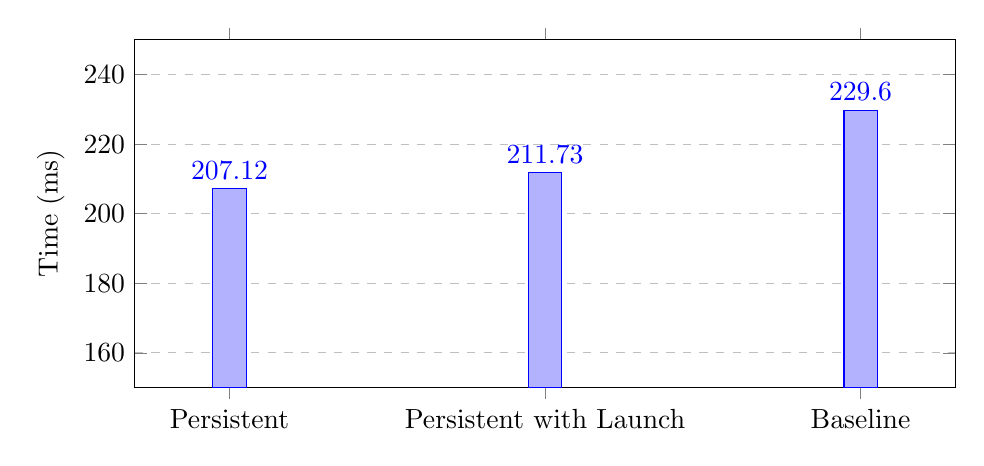
\begin{tikzpicture}
  \begin{axis}[
    ybar,
    bar width=12pt,
    width=12cm,
    height=6cm,
    ymin=150,
    ymax=250,
    ylabel={Time (ms)},
    symbolic x coords={{Persistent}, {Persistent with Launch}, {Baseline}},
    xtick=data,
    nodes near coords,
    nodes near coords align={vertical},
    enlarge x limits=0.15,   % tighter horizontal spacing
    ymajorgrids=true,        % light grid lines for readability
    grid style=dashed,
  ]
    \addplot coordinates {({Persistent}, 207.121) ({Persistent with Launch}, 211.727) ({Baseline}, 229.604)};
  \end{axis}
\end{tikzpicture}


  \caption{Small Kernel and Memory Transfer Tasks}
  \label{fig:sm_sk}
\end{figure}


Figure~\ref{fig:sm_sk} shows the first experiment that was run comparing the task scheduling from the GPU persistent kernel in comparison to the baseline model. 
Here each implementation executes 32 tasks 16x16 matrix multiplication tasks scheduled to the GPU. 
The matrixes for testing are generated at runtime and compared to the correct CPU implementation using the same functios.  

On average over 10,000 runs, the persistent kernel achieved an execution time of 189.165ms, while the baseline model required 229.604ms, demonstrating a clear performance benefit for this small kernel, small memory transfer case.
However, the measurements exhibited high variability, with execution times differing by as much as $\pm$50ms between runs, even averaged over 10000 different executions.
Despite this noise, the persistent kernel consistently outperformed the baseline in the majority of trials.


\subsection{Small Kernel and Larger Memory Transfers}

\begin{figure}[H]
  \centering
  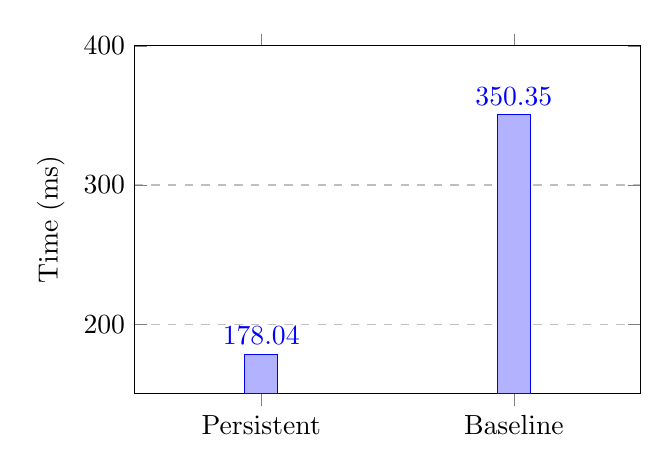
\begin{tikzpicture}
  \begin{axis}[
    ybar,
    bar width=12pt,
    width=8cm,
    height=6cm,
    ymin=150,
    ymax=400,
    ylabel={Time (ms)},
    symbolic x coords={{Persistent}, {Baseline}},
    xtick=data,
    nodes near coords,
    nodes near coords align={vertical},
    enlarge x limits=0.50,   % tighter horizontal spacing
    ymajorgrids=true,        % light grid lines for readability
    grid style=dashed,
  ]
\addplot coordinates {(Persistent, 178.035) (Baseline, 350.349)};
  \end{axis}
\end{tikzpicture}

  \caption{Small Kernel and Larger Memory Transfer Tasks}
  \label{fig:bm_sk}
\end{figure}

In this secondary evaluation, the GPU executes the same task as before but now transfers an additional 1 MiB of memory to the task and returns it.
Interestingly, the persistent thread implementation runs slightly faster than in the previous test, while the baseline control becomes slower.
This unexpected result prompted further testing with a larger input size of 10 MiB, which completed in 623.915ms.

The observed increase in speed is likely due to the underlying memory management strategy.
To conserve valuable GPU resources, the memory buffers are logically partitioned using offsets.
When tasks use very small memory frames, their data ends up placed very close together in memory.
During execution, tasks that read from memory locations adjacent to others simultaneously writing to nearby regions can cause contention and reduce performance.
By increasing the memory size transferred per task, these memory regions are spaced farther apart, reducing contention and allowing the kernel to run more efficiently.

This separation applies to both input and output buffers. 
When transferring larger amounts of data (e.g., 1 MiB or more), the serialized GPU memory transfers no longer interfere with kernel execution, leading to the improved performance observed.

\subsection{Multiple Kernels}



\section{Profiling and Analysis with \texttt{nsys}}

To better understand the execution characteristics of the implementation, \texttt{nsys} profiling was performed for both the baseline (non-persistent) and persistent-threaded approaches. 
In the baseline version, the profiler output is easy to interpret: each kernel launch is explicitly visible on the timeline, interleaved with host-device memory transfers. 
This makes it straightforward to determine where computation occurs, identify launch overheads, and correlate them with memory transfer costs.

In contrast, profiling the persistent-threaded implementation presents significant challenges. 
Since the persistent kernel is launched only once and remains active for the duration of execution, there are no distinct kernel launch entries on the timeline for each individual task. 
Instead, the majority of the visualized activity in \texttt{nsys} consists of frequent host-to-device and device-to-host memory transfers corresponding to the queuing and completion of tasks. 
The actual execution of the tasks within the persistent kernel is effectively "hidden" from the profiler’s high-level view, as it takes place inside the single long-running kernel.

This difference means that the persistent-threaded execution does not lend itself well to the same form of visual, task-by-task inspection available in the baseline case. 
While memory transfer patterns can still be analyzed, the lack of discrete kernel events makes it difficult to directly measure per-task execution time or to distinguish between overlapping computation and data movement. 
To obtain deeper insights, low-level instrumentation or custom device-side logging would be required, as standard profiling tools are optimized for discrete kernel launches rather than continuous, event-driven GPU execution.

Consider the evaluation of the current execution.

\begin{figure}[H]
    \centering
    \includegraphics[width=0.8\textwidth]{data/np_prof.png}
    \caption{Simple \texttt{nsys} timelines for the baseline implementations.}
    \label{fig:nsys_comparison}
\end{figure}





\section{Coroutine Implementation}

While the primary objective of this work was the implementation of GPU persistent threads, it became evident that the same architectural foundations could be extended to support coroutine functionality with relatively modest additional effort. 
The existing design already incorporates a task queue, which the GPU processes in sequence, and a dedicated memory address space for function contexts, making it possible to store and retrieve the continuation state of executing tasks. 
These features naturally lend themselves to coroutine-style execution, where tasks can yield control and later resume from the same execution point.


\subsection{Yielding and Changing Tasks}

In essence, a coroutine yields its execution by voluntarily releasing its currently allocated compute resources, allowing other tasks to make progress. 
Within the present implementation, this can be modeled directly using the existing task queue mechanism. 
The task queue is implemented as a circular buffer, processing tasks in order from the head to the tail. 
When a task yields, it is effectively repositioned within this queue, relinquishing its slot so that another, potentially higher-priority, task can execute in its place. 
The most urgent pending task can then take over the vacated slot, ensuring minimal idle time for the GPU.

A more advanced extension would involve replacing the simple circular buffer with a \emph{priority heap}. 
In such a structure, tasks are automatically sorted and selected for execution based on their priority levels, allowing the scheduler to make more informed decisions about task ordering. 
While the current system executes tasks to completion once they are selected, this model could still allow tasks to voluntarily halt and later resume execution, improving responsiveness for workloads with mixed task lengths.

\subsection{Continuation and Resumption}

Implementing coroutine behavior also requires explicit mechanisms for saving and restoring task state. 
When a task yields, the GPU must store sufficient continuation data so that it can later resume execution from precisely the point where it was interrupted. 
The current memory structure already provides a convenient, per-task memory region where such continuation data can be stored. 
This includes both the computational state and the control information necessary for resuming execution at the correct instruction address within the device function.

To enable this, each task must be preallocated with enough device memory during scheduling to hold both its input parameters and any continuation data that may be required. 
This is achieved by copying the task's input stream into the designated memory region and advancing the memory offset to reserve additional space for storing the continuation state. 
When a task yields, the current execution context—such as register values, loop counters, and program counters—is written into this reserved space. 
Upon resumption, the scheduler retrieves this data and restores the task's execution context, allowing it to continue seamlessly from its previous stopping point. 

By combining these mechanisms with the persistent thread framework, the GPU could effectively execute multiple long-lived, cooperative tasks, enabling finer-grained scheduling and more efficient utilization of GPU resources, especially in irregular or latency-sensitive workloads.


\section{Limitations and Future Work}

The current system does not support priority based scheduling decisions or utilizing coroutines for software preemption like execution.
Future work implementing the strategies outline by this thesis towards utilizing the persistent kernel implemenation as a baseline for these tasks would enable further predictable real time scheduling capabilities. 
In this case, the memory management system might need to progress from an epoch based scheduler to a more complex management system. 
Low priority tasks would interrupt the freeing of epoch memory. 
Furthermore, the current manual streaming of input and output parameters restricts task variability and automation.  
Developing a generalized parameter serialization and deserialization layer that supports arbitrary kernel arguments would increase flexibility and reduce overhead in task preparation.

Further improvements could also include:

\begin{itemize}
    \item Implementing task batching, where each worker processes multiple tasks before polling again, to reduce synchronization overhead.
    \item Optimizing the polling mechanism with adaptive backoff strategies to minimize resource consumption.
    \item Leveraging asynchronous memory copies with double buffering and pinned memory to better overlap data transfers and computation.
    \item Extending the evaluation to more complex kernels and real-world workloads beyond matrix multiplication to better characterize the benefits and limitations of persistent threads.
\end{itemize}

Overall, while the current implementation demonstrates the feasibility of persistent GPU threads, there remains substantial opportunity for optimization and scaling to fully leverage the advantages of this approach.


%If too many tasks are scheduled or the memory buffer becomes fully saturated, task enqueueing fails and the launch function returns a \texttt{-1} error code.  
%Therefore, proper usage requires either a fault-tolerant launching mechanism that can handle task rejections or a carefully designed launch strategy to avoid buffer overflow.
